\begin{abstract}
Public videos attributed to extraterrestrial (ET) channeling are distributed by practitioners, interviewers, archive accounts and repost publishers. A channel crawl can enlarge an index while leaving the speaker, original performance and substantive answer unresolved. This exploratory expansion of Channeling Atlas therefore treats collection, representation and interpretation as separate measurement stages. It preserves the prior \UploadN-upload snapshot, implements practitioner- and entity-aware search and channel collection, audits coverage and publishing concentration, and creates a source-addressable question-answer database from retained digest material. The available Q\&A layer contains \QAN\ AI-digest paraphrase candidates from \QAVideoN\ uploads and one practitioner context; it does not provide cross-practitioner transcript answers. Dictionary extraction and lexical retrieval expose repeated questions and answer vocabulary with source pointers, while the retained caption embeddings support bounded sensitivity diagnostics. New source collection outcomes are reported from actual request logs, including access denials, rather than inferred from installed tools or prepared queries. The resource links an expanded dashboard, executable analyses, generated plots, SQLite/JSON/CSV exports, and a living manuscript. Its contribution is an inspectable bridge from a heterogeneous public-video index to carefully typed analytical units. It does not establish extraterrestrial origins, answer truth, a population census, human construct validation, or independent peer review.
\end{abstract}

\section{Introduction}
An upload title containing ``Bashar,'' ``Ashtar'' or ``Arcturian'' may introduce a live performance, an interview, an old excerpt, a translated repost or a discussion by someone else. A channel name identifies the publisher of that upload; it does not necessarily identify its speaker. A long caption document may contain a host's introduction, audience questions, promotional material and an attributed message. Consequently, computational comparisons become ambiguous when they collapse publisher, practitioner, attributed entity, recording and answer into one unit.

The first Channeling Atlas release addressed this problem through a frozen public-video index, source reconciliation, sampled upload lengths, title and caption representations, and sensitivity checks. The present phase asks how to extend that resource toward richer content analysis without treating search results as a census or summary text as a transcript. The practical brief is broad: investigate channels and materials, collect metadata and offered captions where accessible, search practitioner and entity names, extract keywords, compare questions and answers, and revise the paper and dashboard through additional critical review.

We implement the parts supported by retained evidence and current access. We also make the absent observations visible. In particular, a separately indexed question-answer candidate is useful for retrieval even when its wording is an AI-generated digest paraphrase. It becomes misleading if readers assume a literal spoken question, a verified reply from a named entity, or an answer independently collected from multiple practitioners. Our schema and presentation retain these distinctions at record level.

We organize the expansion around five research questions:
\begin{enumerate}[label=\textbf{RQ\arabic*:}]
\item How concentrated and uneven is the retained upload sample, and which measurement layers remain missing?
\item How do sampled upload duration and visible keyword framing vary together, without inferring complete channel histories or validated content formats?
\item What question-answer material can be indexed with an auditable source and attribution, and what common-question comparisons does it actually support?
\item How do text-layer and publisher dependencies affect the interpretation of the retained representations?
\item Which additional collection and validation steps would discriminate plausible interpretations rather than merely produce larger models or more plots?
\end{enumerate}

The contribution is a reproducible research extension: an explicit search frame and collector, a typed Q\&A database, source-linked keyword extraction, expanded descriptive diagnostics, and a revised evidence explorer and paper. No claim of algorithmic novelty follows from applying TF--IDF, cosine similarity, regular expressions or open-source download software. The proposed methodological value lies in connecting these familiar tools to provenance, abstention and failure states in a small heterogeneous corpus.

\section{Background and Related Work}
\subsection{Matched questions and naturalistic public videos}
Controlled or prospective channeling studies and naturalistic public videos answer different questions. \citet{anastasia2020qualitative} examine elicited content from thirteen trance channels with qualitative methods. \citet{wahbeh2023answers} use scientist-supplied questions and distinguish quantitative correspondence in seven US participants from qualitative work across fifteen participants in two countries. Shared thematic categories in those studies do not establish identical answers, independent information or source verification. Their relevance here is the design emphasis on a question and its context.

The related 2026 prospective semantic and qualitative articles describe a three-channeler program \citep{wahbeh2026semantic,wahbeh2026qualitative}. The retained register distinguishes accessible institutional abstracts and supplement artifacts from unavailable publisher full texts. We therefore use the program as a design comparator for matched prompts, not as an independently reproduced result. An archival study querying two collections through a common AI system introduces another unit: model-generated responses to shared prompts \citep{wahbeh2026records}. Such responses are distinct from a recorded answer and cannot be pooled with our digest candidates or caption vectors.

A genuine cross-practitioner answer study requires more than common vocabulary. It needs comparable prompts, sufficiently complete answer spans, attribution to the answering speaker, treatment of repeated performances, and an explicit relation code such as agreement, qualification, disagreement or indeterminate. Our current Q\&A material does not meet that design for multiple practitioners. This negative scope finding constrains the present results rather than invalidating source-linked indexing.

\subsection{YouTube as a constructed dataset}
YouNiverse demonstrates the importance of documenting how channels and videos enter a metadata resource \citep{ribeiro2021youniverse}. Its scale, thresholds and sampling weights belong to that collection and cannot be inherited by a curated ET-channeling index. Searching every known alias remains purposive selection, and a refreshed URL is not an observation of all uploads on its channel.

Tube2Vec is a close representation precedent: it creates channel embeddings from title and description representations of sampled videos and evaluates representations on human tasks \citep{boesinger2024tube2vec}. Channel centroids and MiniLM are therefore established techniques. Our expansion instead emphasizes the correspondence between record type and permitted interpretation: title resemblance, caption resemblance, paraphrase retrieval and answer agreement remain separate constructs.

Research on religious YouTube content separates narrative, visual and audience dimensions \citep{chen2026digital}. That separation motivates placing each present analysis under a specific question and measurement layer. Studies of platform pathways and content reuse also motivate explicit coding and source tracing \citep{ota2025pathways,starbird2018ecosystem}. Their political or community classifications are not transferred to the people in this corpus. We do not observe viewing paths, recommendation exposure, audience belief or causal influence.

\subsection{Transparent extraction and substantive validation}
Text-as-data research emphasizes that a computational output needs validation for its intended inference \citep{grimmer2013text}. We use explicit keyword dictionaries because readers can inspect a rule, a matched record and a denominator. Transparency does not establish semantic validity: a match can be metaphorical, negated, quoted or a host's language, while an unmatched synonym can express the same idea.

Topic-model studies distinguish interpretability, coherence and reliability \citep{chang2009reading,doogan2021twaddle,hoyle2021incoherence,schroeder2025reliability}. Newer work on large-language-model topic descriptions likewise warns that fluent summaries can remain generic without domain participation \citep{li2025haystack}. We therefore do not rename dictionary counts ``validated topics,'' infer a speaker's position from a theme label, or treat model-agent agreement as a reliability statistic.

Sentence-BERT provides an established basis for separately encoded sentence comparison \citep{reimers2019sentencebert}; embedding benchmark results remain task- and language-dependent \citep{muennighoff2023mteb,enevoldsen2025mmteb}. The inherited pinned MiniLM features are an auditable baseline, not a claim of current best performance. Alternative encoders, topic models, speech recognition and keyword-ranking packages are distinguished as executed, inspected or proposed in the software register.

\subsection{Source access and literature scope}
This is a targeted related-work update, not a systematic review. The prior 28-source register retains reading locations and access depth. This phase additionally records actual source requests and software README/license retrieval. A denied publisher request is an access observation; it does not show that the article is absent or that a cited method has been reproduced. Software documentation establishes supported features and caveats, not scientific validation on this discourse.

\section{Data, Identity and Evidence Layers}
\subsection{Preserved baseline and new extension}
The scientific baseline is the reviewed October 2026 snapshot preserved at GitHub commit \texttt{bbe4801}; the continuation handoff is \texttt{1d6eb36}. Full commit identifiers and input hashes are recorded in the source manifest. The former paper, data, plots and reviews remain intact. This extension writes new artifacts and fresh review records. Historical review receipts are evidence about their original files, not certificates for this manuscript.

The inherited union combines 482 atlas video identifiers with 457 valid unique archive identifiers, of which fourteen overlap, producing \UploadN\ unique uploads. Nine archive rows without a usable identifier remain leads. The source directory contains account routes, aliases and unresolved records, rather than a count of unique humans. Refreshed watch-page metadata and explicitly labeled inherited values supply duration and date fields. The new diagnostics recompute summaries from that frozen evidence unless an explicitly logged collection result is identified.

\begin{table}[htbp]
\small\centering
\setlength{\tabcolsep}{4pt}
\begin{tabular}{p{0.43\textwidth}p{0.13\textwidth}p{0.14\textwidth}p{0.14\textwidth}}
\toprule
Measurement layer & Available & Indexed pool & Share \\ \midrule
Publishing account resolved & 886 & 925 & 95.8\% \\
Positive upload duration & 881 & 925 & 95.2\% \\
Exact upload date & 880 & 925 & 95.1\% \\
English-likely eligible title & 742 & 925 & 80.2\% \\
Frozen English caption pilot & 30 & 925 & 3.2\% \\
\bottomrule
\end{tabular}
\caption{Inherited snapshot coverage. The caption row is selected pilot inclusion, not estimated caption availability. Denominators describe known uploads.}
\end{table}


\subsection{A typed identity model}
We distinguish (1) a human practitioner, (2) a publishing account, (3) a YouTube upload, (4) an original performance/session, (5) a text artifact or derived record, and (6) a publicly attributed entity label. These relationships are many-to-many. A practitioner may appear on several interview accounts. One account may host several practitioners. One performance can be edited into several uploads, and one attributed label can be used by more than one human.

Only explicit source-supported aliases are merged. A matching first name or entity term is insufficient. Records retain unresolved identity links and adjacent spiritual or historical material. This prevents discovery coverage from becoming a misleading active-medium count. Original-session grouping remains incomplete; exact upload-ID deduplication and repeated-title exclusion are deliberately narrower operations.

\subsection{Metadata, captions and digest paraphrases}
The baseline provides \DurationN\ usable durations, \DateN\ exact upload dates and \TitleN\ eligible titles within the known index. These describe the indexed records, not the full platform. Publication dates can date reposts rather than performances. Language decisions on short titles are heuristic, and titles are publisher framing rather than complete speech.

The retained caption pilot attempted 36 uploads, retrieved 34 tracks and retained 30 English documents in the balanced analysis. Thirty-two of the retrieved tracks are platform-labeled automatic and two are platform-labeled manual; the manual flag is not an accuracy audit. None was audio-corrected or speaker-diarized. Numeric derivatives are retained, but raw captions and model weights are absent from the public checkout. This extension does not claim that those derivatives recreate transcript text or that new raw-caption inference has occurred.

The Q\&A source layer is different again. Its \QAN\ candidates come from \QAVideoN\ Q\&A-bearing digests among 75 retained AI-generated digests of Darryl Anka-related uploads. They contain question paraphrases and answer gists, not verbatim turns. Some source videos are interviews, clips or mixed formats. We preserve their practical discovery value while setting speaker verification to false and withholding invented timestamps or exact quotations.

\section{Methods}
\subsection{Search, channel crawling and acquisition status}
The collection plan expands names into explicit query records rather than hiding search choices in an informal browsing history. Its units include practitioner names, documented aliases, attributed entity terms and account URLs. The implemented query templates combine a quoted name with \emph{channeling}, \emph{questions answers}, or \emph{interview}, plus quoted name/entity combinations when the entity label differs from the name. Each planned query has its rationale and scope; entity names are discovery terms rather than proof of attribution. Per-account caps and a fixed ordering make the selected subset reviewable. Search-result ranks remain platform outputs at a time, not stable inclusion probabilities.

The collector uses ordinary public endpoints and open-source software. \texttt{yt-dlp} supports flat channel/search metadata enumeration without media acquisition; flat results can omit details, so a flat record is not silently promoted to complete watch metadata. \texttt{youtube-transcript-api} retrieves offered caption tracks and records language and automatic/manual flags. Runtime source and version manifests distinguish an installed package from a successfully executed acquisition operation. Where a metadata date is approximate, it remains approximate.

Access outcomes are explicit. The current environment's restricted outbound policy denied ordinary YouTube watch requests with a proxy tunnel HTTP 403. Required domains were saved to the environment configuration draft; that action did not apply the policy or create successful crawls. Collector preflight and failure manifests preserve the difference between a prepared query, an attempted request, an unavailable caption and a successful artifact. A policy denial is not evidence that a video is deleted or that its channel has no speech.

No proxy rotation, cookies, paywall circumvention, CAPTCHA bypass or private-account access is used. Suggestions in third-party software documentation to rotate residential proxies are not adopted. A supported public API with a properly scoped credential is an alternative collection route if later configured; no API access is assumed in this release. The client environment already routes HTTPS through its session proxy, a transport arrangement distinct from rotating exit identities to evade a denial.

\subsection{Keyword extraction and denominators}
We report keyword-based extraction explicitly in both methodology and record-level outputs. The nine retained theme families cover contact/disclosure, agency/beliefs, healing, consciousness, energy, society, relationships, practice, and time/realities. Their executable regular expressions are retained. Additional Q\&A extraction applies theme and answer-modality rules separately to the question paraphrase and answer gist. Overlapping families can match a single record; their counts must not be summed as a partition of content.

For document $v$ and dictionary family $t$, title presence is
\begin{equation}
 I_{vt}=\mathbb{1}\{\text{at least one documented expression from }t\text{ matches the title}\}.
\end{equation}
Within a duration band or account, the presence share divides the number of matched eligible titles by the eligible titled uploads in that group. The caption rate is a separate quantity, the number of matches per 1,000 tokenizer-defined words. Neither quantity is a percentage of time devoted to a theme. Question and answer counts likewise have distinct text opportunities. A difference between long captions and short titles can arise mechanically because long text offers more chances to match.

The rules preserve an inspectable baseline and candidate retrieval path. They do not resolve negation, sarcasm, quotation, speaker identity, ontology, correctness or comprehensive theme prevalence. Keyword candidates guide close reading; they do not replace it. We retain examples that challenge the codebook and leave unmatched records as unmatched rather than inventing a catch-all interpretation.

\subsection{Source-addressable Q\&A database}
Each candidate has a stable identifier, video identifier, source URL, source file SHA-256, JSON pointer, question paraphrase, answer gist, publisher fields, contextual practitioner/entity fields, evidence type and verification state. The version-1 schema specifically describes inherited digest candidates; it is not a generic schema of verified transcript turns. SQLite provides structured queries and joins; JSON and CSV support inspection and exchange. Source hashes and pointers make a result traceable to a particular retained digest revision. Null timestamps are meaningful missing data and do not become zeros.

Exact wording is not treated as original speech. The evidence type is \texttt{ai\_digest\_paraphrase}; a candidate may be useful while its literal transcript turn remains unavailable. Publisher attribution resolves where an upload appears. Practitioner context describes the digest corpus, and an entity label describes its source framing. Neither automatically confirms the answer speaker. Cross-practitioner answer analysis remains unavailable in this source layer because all retained candidates concern one practitioner context.

Common-question retrieval uses lexical representations of question paraphrases. Question and answer-gist matrices are fitted separately with word unigrams/bigrams, English stop words, minimum document frequency one, sublinear term frequency, smooth inverse-document frequency and L2 normalization. All question pairs from distinct upload IDs with cosine at least 0.40 are retained; this is a retrieval cutoff, not a calibrated semantic equivalence threshold. Let $x_i$ be the TF--IDF vector of candidate question $i$. Candidate neighbors are ordered by
\begin{equation}
 s_{ij}^{(Q)}=\frac{x_i^\top x_j}{\lVert x_i\rVert_2\lVert x_j\rVert_2}.
\end{equation}
The corresponding answer-gist score $s_{ij}^{(A)}$ is computed separately. A high question score indicates shared wording under this representation; a high answer score indicates shared answer vocabulary. Neither measures agreement, completeness or truth. Near-identical formulas can produce high scores while substantively distinct qualifications remain important. Scores from the same upload are separated from cross-upload candidates, and no lexical threshold is relabeled as a calibrated match probability.

\subsection{Model-assisted close reading}
The extraction review examines selected source digests and candidate neighbors against their question and answer-gist fields. Reviewers record why a pair is topical, formulaic, contextually ambiguous or unsupported. These are model-assisted interpretations of summaries. They are not blinded human annotations, inter-rater agreement estimates, a transcript accuracy audit or direct audiovisual observation. A useful disagreement between code and reading is retained as a limitation and a codebook correction candidate.

The next empirical annotation phase should preserve the prompt and full answer window, mask model rank where appropriate, and code at least topical overlap, proposition agreement, qualification, disagreement and indeterminate. Human coders should receive an explicit codebook and a held-out adjudication set. That work is proposed, not retrospectively claimed here.

\subsection{Coverage, concentration and duration diagnostics}
Coverage is measured at the unit actually observed. For a field $f$, the missing share is $1-n_f/N$, where $N$ is the relevant indexed pool. Publisher-level caption selection is distinguished from upload-level availability; failure in a small selected pilot cannot estimate all-channel caption access.

For attributed uploads, publisher concentration is summarized by shares $p_c=n_c/\sum_c n_c$, the Herfindahl concentration $\sum_c p_c^2$, effective publisher count $1/\sum_c p_c^2$, and cumulative leading-account shares. These describe how much a few publishing routes contribute to the retained sample. The measures do not identify media influence or practitioner prevalence.

Duration bands summarize observed upload length. They are named by minutes rather than assumed genres. Long recordings can still be interviews or compilations, and short recordings can contain substantive answers. Associations between duration and dictionary presence use eligible titles and expose their denominators. Caption selection contrasts use deterministic empirical quantiles; no caption-selection resampling was performed. The new publisher-label negative controls use the fixed seed and unit documented in the executable protocol. Historical balanced title resampling remains a separately recorded prior analysis. All outputs are scoped to the retained sample; sampling bias and unresolved performance reuse remain.

\subsection{Retained representations and sensitivity}
The inherited encoder is the pinned \texttt{all-MiniLM-L6-v2} ONNX CPU model. Caption processing uses deterministic chunks and explicit normalization; public numeric outputs allow recalculating comparisons, while source-text re-inference requires local authorized captions and verified model artifacts. Within- and between-publisher pair scores share documents and therefore are dependent. Account-pair counts are not independent participant counts. Equal-account summaries first average within each eligible account and between each eligible account pair, then compare those averages. They address weighting of the observed sample; they do not create human-level independence. Leave-one-publisher-out ranges remove a publisher and its incident pairs and quantify influence, not confidence intervals.

The prior matched title/caption comparison uses the same 22 videos from eleven accounts, yielding 55 account pairs. Boundary trimming, name/genre masking, title-string exclusion, balanced sampling and token-weighted pooling perturb different decisions. A stable global ordering can coexist with a changed nearest neighbor. These comparisons are descriptive diagnostics and do not establish speaker signatures or attributed-entity communication.

\section{Results}
\subsection{Implemented collection and observed access}

The new plan contains 106 inherited practitioner/lineage/partial-name candidates, 590 planned keyword queries, 157 planned account crawls and 215 proposed caption candidates, alongside 925 retained upload IDs. These are different units and are not additive. The recorded initial preflight attempted 1 ordinary watch request and observed 1 policy block; newly successful collection operations total 0. Therefore no new search results, channel histories, metadata records or captions are added by this collection phase.

The installed collector dependencies are \texttt{yt-dlp 2026.10.21} and \texttt{youtube-transcript-api 1.2.4}. The observed watch preflight used Python standard-library \texttt{urllib}; no successful tool-backed crawl or caption retrieval occurred. Package import and dependency checks establish local availability, while mocked safety tests establish selected control behavior; neither is successful platform retrieval. The documented query forms are quoted practitioner name with \emph{channeling}, \emph{questions answers}, or \emph{interview}, plus documented name/entity combinations. Other spelling variants are proposed sensitivity checks.

\subsection{Coverage and publisher concentration}

Of 925 retained uploads, 886 resolve to 180 nonempty publisher groups, while 39 remain unresolved. The largest ten groups contribute 38.04\% of attributed uploads; the largest twenty contribute 66.93\%. Thus the exploratory direction check that the largest ten exceed half is disconfirmed in this sample. These checks were recorded after inspection of the schema and prior summaries, before the new computations; they are not preregistered. The upload-count Gini is 0.671; inverse-Herfindahl effective representation is 40.30 equally sized groups. These are sample concentration measures, not audience or practitioner statistics.

\begin{figure}[p]
\centering
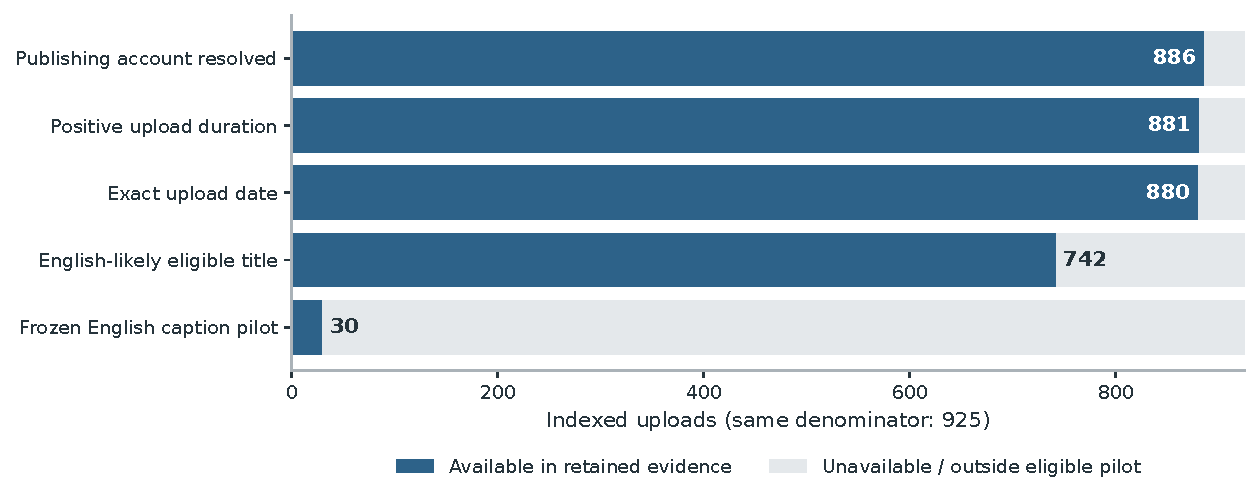
\includegraphics[width=\textwidth]{generated/figures/coverage.pdf}
\caption{Availability of retained measurement layers. The selected caption-pilot row is inclusion in this released pilot, not a census of offered-caption availability. Missing observations are not negative content findings.}
\label{fig:coverage}
\end{figure}

\begin{figure}[p]
\centering
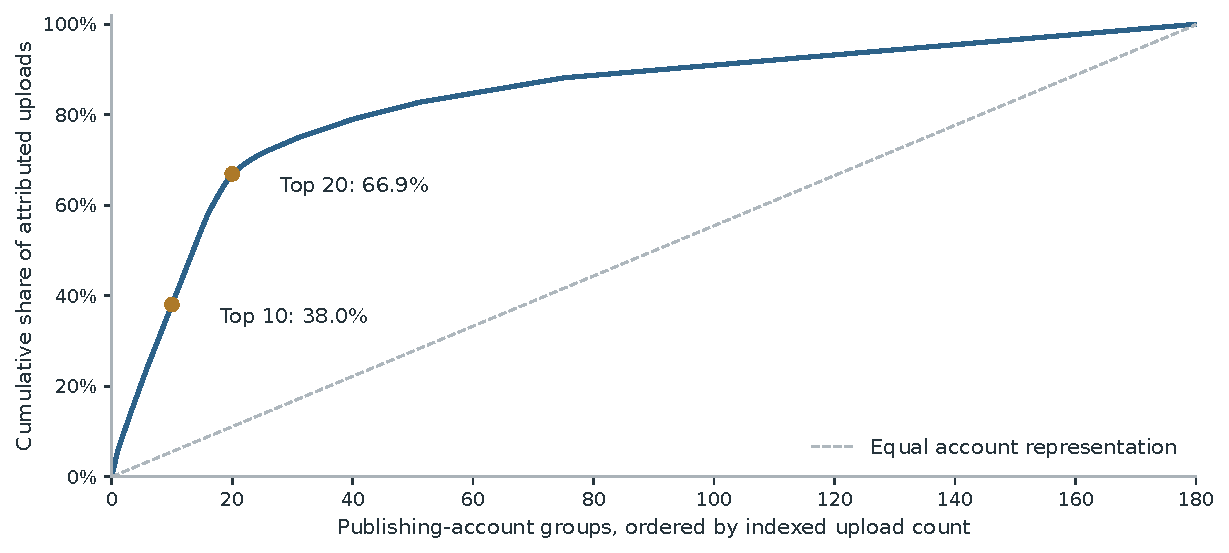
\includegraphics[width=\textwidth]{generated/figures/concentration.pdf}
\caption{Publishing-account concentration among attributed retained uploads. Ranks and cumulative shares describe sample composition. They do not measure followers, views, influence or unique human practitioners.}
\label{fig:concentration}
\end{figure}

\subsection{Caption selection does not favor longer recordings in this snapshot}

The 30 English pilot uploads have median observed length 8.61 minutes, compared with 19.37 minutes in the other 851 indexed uploads with known duration. Restricting the comparison to the pilot's 17 publisher groups gives median 12.04 minutes among 430 other known-duration uploads. The pilot therefore does not have a larger median in either descriptive contrast. This disconfirms the proposed longer-pilot direction, but it is not an estimate of how duration causes caption availability: the pilot selection was purposive and its failures were limited.

\begin{figure}[p]
\centering
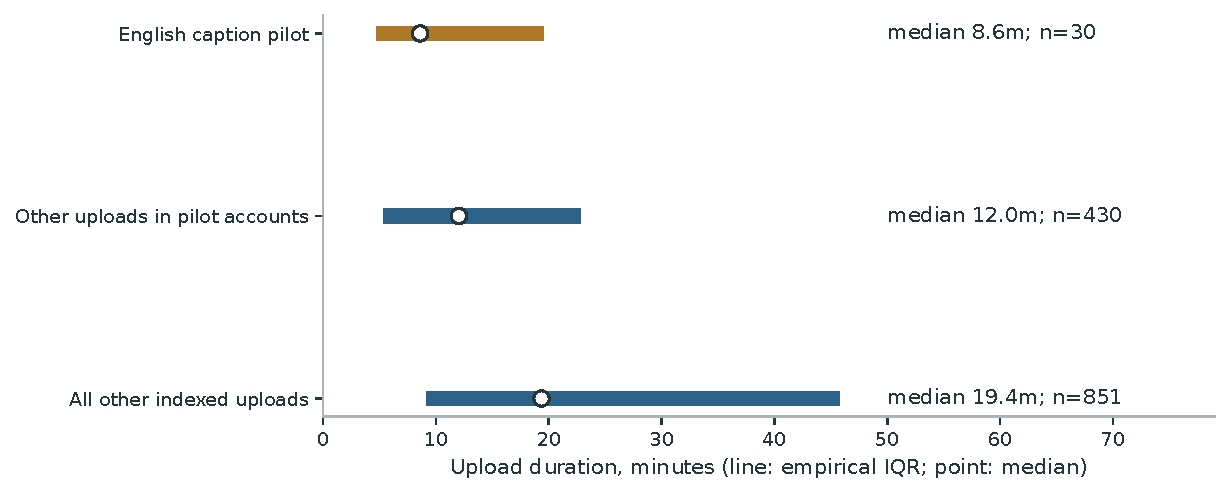
\includegraphics[width=\textwidth]{generated/figures/caption-selection.pdf}
\caption{Observed duration distributions for the English caption pilot, other indexed uploads, and other uploads from pilot publishers. Quartile spans describe observed records; they are not confidence intervals or corrected population estimates.}
\label{fig:caption-selection}
\end{figure}

\subsection{Length and title-keyword framing depend on aggregation}

The title/duration diagnostic uses 702 eligible titles with measured duration: 431 uploads shorter than thirty minutes and 271 of at least thirty minutes. Only 11 accounts meet the paired-account rule on both sides. The pooled direction agrees with the paired-account median direction in two of nine dictionary families. Six paired medians are exactly zero; they must not be described as six reversed effects.

The society/world-events family illustrates an actual sign change: its pooled long-minus-short presence contrast is +4.89 percentage points, whereas the median paired-account contrast is -4.55 points. The compared pools and weighting differ; this is evidence to inspect composition, not a causal duration effect or a full Simpson-paradox identification.

\begin{table}[htbp]
\small\centering
\setlength{\tabcolsep}{4pt}
\begin{tabular}{p{0.39\textwidth}p{0.19\textwidth}p{0.22\textwidth}p{0.08\textwidth}}
\toprule
Dictionary family & Pooled long--short, pp & Median account contrast, pp & Groups \\ \midrule
ET contact \& disclosure & +2.82 & +0.00 & 11 \\
Choice, beliefs \& manifestation & +0.43 & +0.00 & 11 \\
Healing \& wellbeing & -3.26 & +0.00 & 11 \\
Consciousness \& awakening & -0.74 & -4.55 & 11 \\
Energy \& frequency & -5.70 & -3.33 & 11 \\
Collective \& world events & +4.89 & -4.55 & 11 \\
Love \& relationships & -1.21 & +0.00 & 11 \\
Meditation \& practice & -1.12 & +0.00 & 11 \\
Time, dimensions \& realities & +6.50 & +0.00 & 11 \\
\bottomrule
\end{tabular}
\caption{Duration contrast among eligible titles. Families overlap. Per-account estimates use the separately eligible paired-account subset; a zero median is not a directional reversal.}
\end{table}


\begin{figure}[p]
\centering
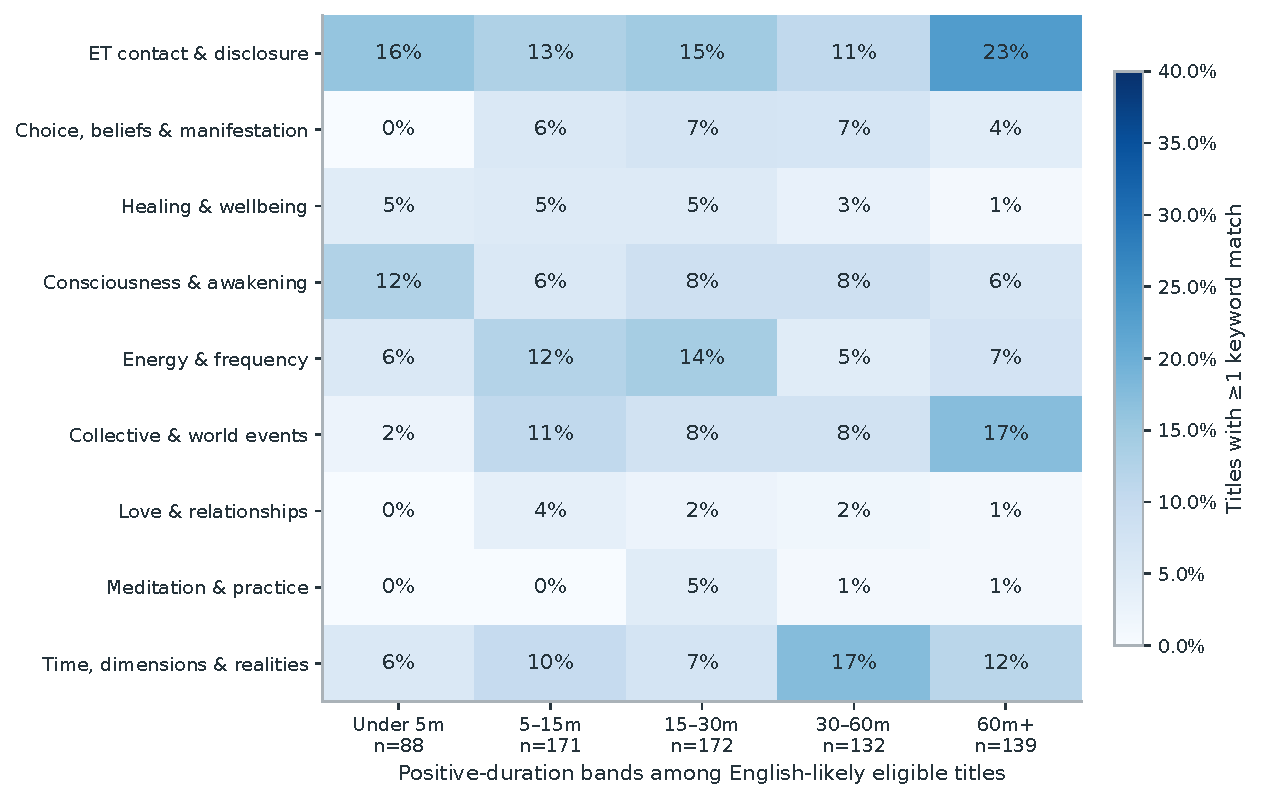
\includegraphics[width=\textwidth]{generated/figures/keyword-duration.pdf}
\caption{Title dictionary presence by observed upload-duration band. Cell denominators are eligible titled uploads with measured duration. Keywords indicate visible framing, not time spent on a theme or validated spoken content.}
\label{fig:keyword-duration}
\end{figure}

\subsection{Publisher resemblance remains a descriptive property of text}

The new upload-pair diagnostic intersects the existing title and caption derivatives, yielding 25 uploads from 14 publishers. This includes groups that do not meet the older two-document account-centroid threshold, so it differs from the prior 22-video/eleven-account centroid comparison. Both new text-layer diagnostics use the same 25 uploads. The mean same-publisher minus different-publisher cosine is 0.154 for captions and 0.229 for titles. The scores describe resemblance under fixed representations, not the probability of shared authorship, an attributed entity or answer agreement.

There are 11 same-publisher and 289 different-publisher upload pairs; 11 accounts have a within-account pair and 3 accounts are singletons. An equal-account sensitivity gives separation 0.153 for captions and 0.229 for titles across 11 eligible focal publishers. Omitting each publisher in turn gives caption separation 0.121--0.179 and title separation 0.186--0.259. These deterministic influence ranges are not confidence intervals.

Caption minus title pooled separation is -0.075; its equal-account analogue is -0.075. Cosine scales are representation-specific, so the difference is a descriptive sensitivity rather than a calibrated amount of semantic or practitioner signal.

The label-shuffle reference permutes publisher labels on the fixed vectors while preserving group sizes (2,000 seed-42 permutations). It is a descriptive negative control, not a population p-value or independent-pair confidence interval. Unresolved original-session reuse, account boilerplate, hosts and publisher formatting remain explanations for a within-publisher advantage. A failure to resemble arbitrary shuffled labels does not isolate a practitioner mechanism.

\begin{figure}[p]
\centering
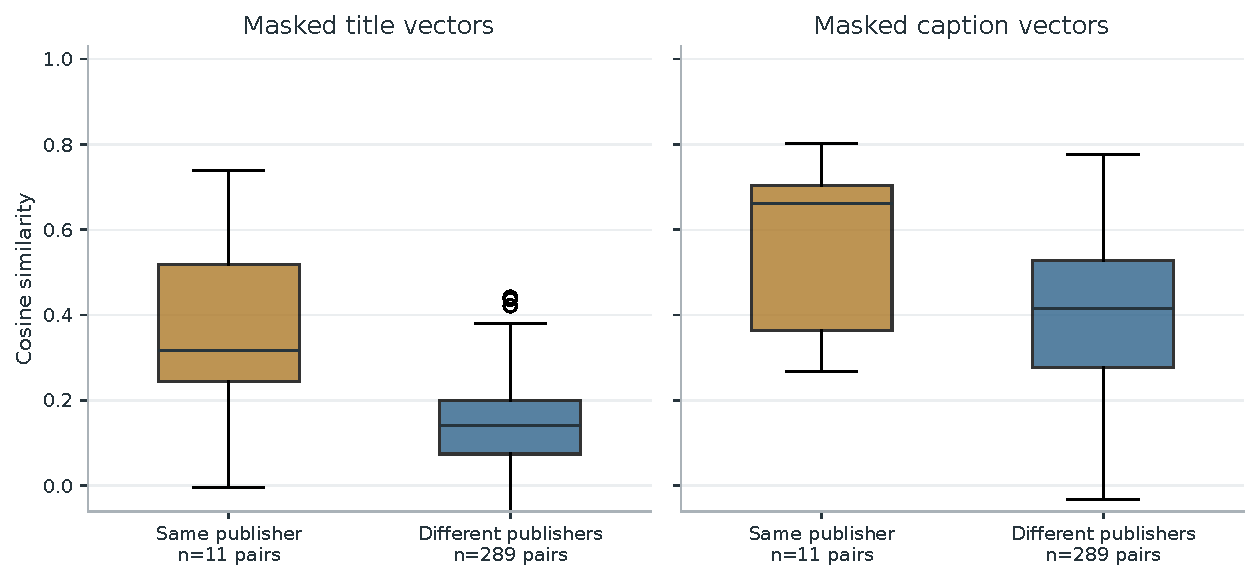
\includegraphics[width=\textwidth]{generated/figures/publisher-similarity.pdf}
\caption{Same- versus different-publisher cosine summaries on fixed title and caption derivatives. Pair entries reuse uploads and are dependent. The new matched upload pool differs from the earlier thresholded centroid cohort.}
\label{fig:publisher-similarity}
\end{figure}

\begin{figure}[p]
\centering
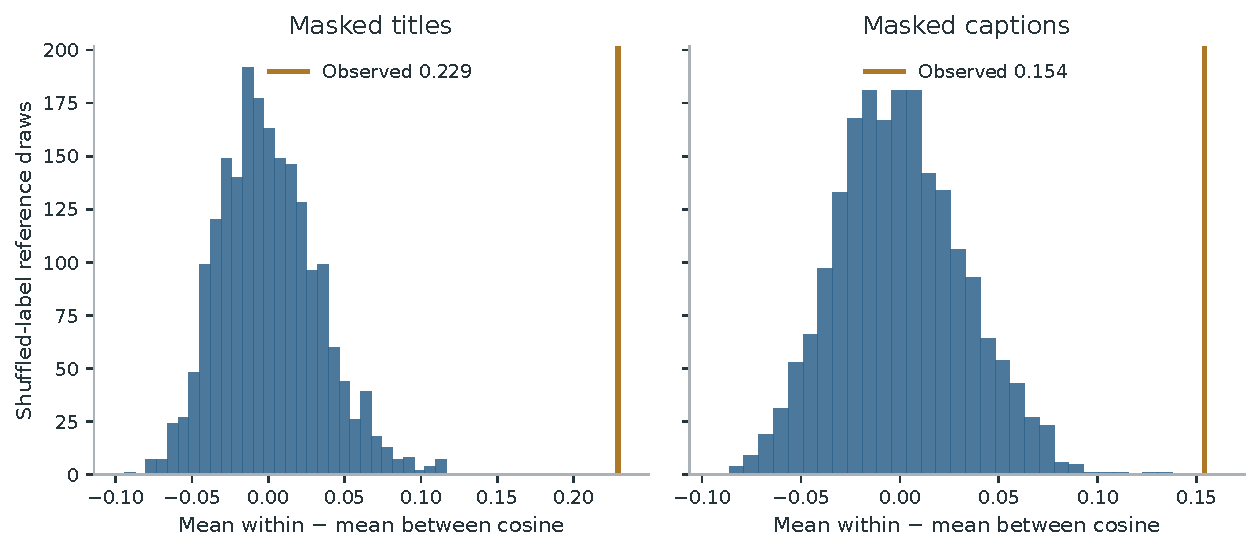
\includegraphics[width=\textwidth]{generated/figures/negative-control.pdf}
\caption{Fixed-vector publisher-label shuffle reference. Labels are permuted with group sizes preserved. The distribution is a descriptive diagnostic, not a population null distribution, a calibrated p-value or evidence about communication origin.}
\label{fig:negative-control}
\end{figure}

\subsection{Repeated title strings are not original-session families}

The new explicitly normalized eligible-title audit finds 2 repeated-string families involving 4 documents among 742 eligible titles; none spans different resolved publishers. Its normalization is different from the inherited embedding-deduplication pipeline. The inherited pipeline's pair-order correlation after its own exclusion rule is 0.992, while raw versus name/genre-masked title rankings correlate at 0.626. These are distinct operations and counts. Neither audit establishes that differently titled uploads are different original performances.

\subsection{Question-answer candidates: useful retrieval, one practitioner context}

The database indexes all 949 retained question/answer-gist entries from 67 Q\&A-bearing digests among 75 source digests. All belong to one Darryl Anka-related practitioner context. They span 27 resolved publisher IDs; 105 candidates lack a resolved publisher ID and remain in 7 inherited-name groups. There are 0 literal transcript turns, 0 verified answer-speaker candidates, and 0 human-reviewed candidates in this layer. The other inherited practitioner candidates do not acquire Q\&A rows merely because they appear in the discovery frame.

\begin{table}[htbp]
\small\centering
\setlength{\tabcolsep}{4pt}
\begin{tabular}{p{0.48\textwidth}p{0.23\textwidth}p{0.15\textwidth}}
\toprule
Source-digest format & Q\&A-bearing uploads & Candidates \\ \midrule
Q\&A only & 5 & 35 \\
clip & 6 & 25 \\
interview with Darryl Anka & 20 & 353 \\
monologue+Q\&A & 36 & 536 \\
\bottomrule
\end{tabular}
\caption{Inherited digest format labels among Q\&A-bearing uploads. Labels are retained source metadata, not a newly validated format taxonomy or answer-speaker annotation.}
\end{table}


\begin{table}[htbp]
\small\centering
\setlength{\tabcolsep}{4pt}
\begin{tabular}{p{0.49\textwidth}p{0.18\textwidth}p{0.2\textwidth}}
\toprule
Q\&A dictionary family & Question matches & Answer-gist matches \\ \midrule
ET contact and disclosure & 155 & 165 \\
Excitement and life direction & 55 & 115 \\
Beliefs, emotions and relationships & 78 & 188 \\
Consciousness and parallel realities & 160 & 348 \\
Channeling and spiritual practices & 89 & 148 \\
Body, health and physical claims & 82 & 265 \\
Time windows and predictions & 31 & 51 \\
History, society and institutions & 42 & 125 \\
\bottomrule
\end{tabular}
\caption{Overlapping keyword matches in question paraphrases and answer gists. Both columns use 949 candidates but different text fields and lengths. Counts are neither validated themes nor measures of agreement.}
\end{table}


There are 936 unique normalized question strings and 11 repeated-string groups. Across distinct uploads, 127 question pairs meet the lexical cosine threshold of 0.40. Excluding identical normalized question wording leaves 112 pairs. These are candidate retrievals, not independent question occurrences or evidence that separate original sessions answered the same prompt.

The retrieval count is sensitive to its exploratory cutoff: increasing question cosine from 0.40 to 0.90 reduces candidate pairs from 127 to 18. At 0.40, the 127 candidate matches occupy 71 distinct upload pairs; the three leading upload pairs supply 30 matches (23.6\%). Concentration can reflect shared questions, reused original material or summary normalization. It is not an observed repost rate or an independent-session count.

\begin{table}[htbp]
\small\centering
\setlength{\tabcolsep}{4pt}
\begin{tabular}{p{0.31\textwidth}p{0.29\textwidth}p{0.27\textwidth}}
\toprule
Minimum question cosine & Candidate question pairs & Distinct upload pairs \\ \midrule
0.40 & 127 & 71 \\
0.50 & 73 & 34 \\
0.60 & 47 & 19 \\
0.70 & 34 & 11 \\
0.80 & 24 & 11 \\
0.90 & 18 & 9 \\
\bottomrule
\end{tabular}
\caption{Exploratory lexical retrieval sensitivity. These thresholds recount the retained question candidates and are not validated equivalence cutoffs. Distinct upload pairs can still share an original performance.}
\end{table}


The summary preview displays 100 of the 127 retained pairs; the complete records are in \texttt{question-pairs.json} and SQLite. Preview truncation is not a lower analyzed denominator. CSV verification/speaker fields retain explicit false values rather than blank strings; null timestamps still mean that no precise turn time is available.

One retrieved pair repeats the digest question \emph{Do we have one life purpose or many?} across two uploads. Its question cosine is 1.000 but its answer-gist cosine is 0.346. The source relation is unresolved: this could involve distinct explanations, summary wording or shared original material. The database correctly marks answer agreement as not assessed rather than converting either score into an agreement verdict.

Twenty deterministically selected digest candidates received model-assisted close reading. The review observes that a contact-oriented question can receive an excitement/formula answer; nested reported speech is not a direct entity turn; precise dates and percentages remain attributed assertions; and a physical-claims keyword is not a clinical validation. The inspected material was the retained question/gist fields. No reviewer listened to the audio or inspected a new transcript in this phase, and the twenty readings do not establish accuracy or inter-rater agreement.

A subsequent purposive paired reading inspects 12 high-question-similarity examples, selecting the first distinct left-question strings in descending cosine order. The model annotations identify compatible paraphrases with low answer-gist cosine, different facets that are not necessarily contradictions, and possible repeated source families. For example, the question of preparing for contact receives passion/formula/vibration advice in both summaries despite low lexical answer similarity. Another pair uses a relative time window versus calendar windows; without original recording dates, it cannot establish chronological drift. Every answer-agreement field remains undetermined. These selected examples refine interpretation of retrieval, not its representative accuracy.


\section{Interpretation}
\subsection{A richer index is useful before it becomes an answer study}
The Q\&A extension makes a concrete contribution: readers can retrieve question paraphrases, inspect answer gists, follow source pointers and distinguish thematic repetition from absent observations. This reduces the temptation to ask an unrestricted model to reconstruct answers from channel names alone. It also exposes the largest design gap: the available candidate source does not contain independently collected answers from multiple practitioners. A multi-medium comparison cannot be recovered by treating interview publishers as separate mediums.

Within one practitioner context, recurring questions can still be studied. A cluster of questions about beliefs or contact may reveal repeated audience concerns in this digest selection. It does not reveal how often all viewers ask such questions, and the source summarizer may have normalized diverse wording into similar paraphrases. Answer-gist similarities may therefore reflect both discourse and the digest production process. The separate question and answer fields support testing this alternative once original spans are available.

\subsection{Publishing form competes with substantive interpretation}
The duration and coverage diagnostics put platform presentation before claims about content. A collection dominated by a few publishers or by short extracts can produce a strong account-level signature without a stable speaker-level difference. Longer uploads can mix questions, answers, hosts and promotions; shorter titles have fewer opportunities for dictionary matches. Same-session reuse can create apparently independent similarities across accounts.

Consequently, an observed relation between length and keywords remains a result about sampled upload framing. An observed within-publisher embedding advantage can result from account-specific editing, recurring hosts, boilerplate or repeated source recordings. A disconfirming comparison should match duration and format, group original performances, and annotate answer speakers. It should not merely add more pairwise scores from the same records.

\subsection{What the new tools change}
Open-source collection and analysis tools improve reproducibility when their operation, version and failure states are retained. They do not remove access controls, grant redistribution rights or validate a theoretical construct. A reproducible denial is preferable to a silently fabricated transcript. A reviewed README is not an executed model, and an installed model package is not evidence that its weights, transcript outputs or accuracy were evaluated.

The present system therefore supports two branches. The evidence branch analyzes retained public metadata and derivative features, producing new exact tables and plots. The acquisition branch implements a repeatable process and preserves denied or not-attempted records until supported access is available. The paper and dashboard show both branches without combining their counts.

\section{Novelty, Alternative Explanations and Limits}
\subsection{What is contributed and what is established practice}
TF--IDF, dictionary matching, caption retrieval, channel centroids and SQLite are established methods. We do not claim the first computational study of channeling, the first YouTube channel embedding or a novel agreement detector. The proposed contribution is an evidence-typed integration: a frozen heterogeneous index, auditable source precedence, question-answer candidates with explicit paraphrase status, transparent retrieval, selection diagnostics and linked review artifacts.

The contribution is a working research resource rather than a new empirical result about communication origin. A broader literature search may identify closely comparable resources. Failed access does not justify priority claims, and future publication must assess the contribution against relevant domain, social-computing and information-retrieval work.

\subsection{Main threats to interpretation}
\textbf{Selection and coverage.} The frame is purposive, historically mixed and influenced by search visibility and archive caps. Inclusion probabilities are unknown. Crawling known accounts more fully would improve within-account coverage but would not create a census of practitioners. Unresolved names and publisher aliases limit cross-account attribution.

\textbf{Summarization and recognition.} Digest questions and answer gists were AI-generated from public recordings. They may omit qualification, normalize vocabulary or misattribute speech. The caption pilot is mostly automatic, uncorrected and undiarized. No present result establishes word error rate, speaker accuracy or transcript completeness.

\textbf{Measurement and dependence.} Dictionary families overlap and are not validated topics. Word counts, title presence, caption rates and duration bands answer different questions. Pair scores share documents; repeated performances may persist after upload-ID deduplication. Model-assisted review is not independent human evidence.

\textbf{Temporal interpretation.} Upload date is not performance date or a live-activity observation. Earlier service offers and prices have separate cutoffs and are not refreshed by this analysis. Indexed monthly counts do not establish channel posting rates.

\textbf{Access and reproduction.} The public release omits raw captions and weights. Frozen-feature reproduction and complete source-text/model recomputation are different capabilities. New collection is blocked until the environment's required destinations are applied and tested. Access may still fail afterward for platform-specific reasons.

\textbf{Physical or psychological claims.} Similarity is not evidence for an extraterrestrial source, truth, independence of information or clinical condition. The study describes publicly attributed claims without endorsing their origin or diagnosing practitioners or audiences.

\section{A Falsifiable Research Agenda}
Future work is organized around contrasts that can fail, rather than a list of fashionable models.
\begin{enumerate}
\item \textbf{Prompt equivalence.} Collect actual question and complete answer spans across practitioners. Compare retrieved pairs with blinded human judgments. The hypothesis that high lexical neighbors are equivalent prompts fails if most are judged materially different or underspecified.
\item \textbf{Answer relations.} Given matched prompts, code agreement, qualification, disagreement and indeterminate separately from topical overlap. The hypothesis that high answer cosine signals agreement fails if its held-out discrimination does not exceed a documented lexical baseline.
\item \textbf{Publisher versus practitioner.} Sample practitioners appearing on multiple accounts and accounts hosting multiple practitioners; use matched formats and original-session groups. A practitioner-specific signal fails if publisher/host labels explain equal or greater held-out resemblance after leakage controls.
\item \textbf{Host and promotion segmentation.} Compare whole-upload and speaker/context windows on identical recordings. The hypothesis that attributed-message windows improve substantive neighbor quality fails if blinded relevance is unchanged or worse, including uncertainty intervals and exclusions.
\item \textbf{Original-session reuse.} Group edits and reposts using explicit source relationships and authorized audiovisual evidence. A claimed cross-account relation fails as independent evidence when it is explained by repeated performances.
\item \textbf{Multilingual and model comparisons.} Evaluate at least one licensed contemporary encoder on the same human-reviewed items, with language-specific reporting and resource constraints. A leaderboard advantage is irrelevant if in-domain pair judgments do not improve.
\item \textbf{Keyword validation.} Sample matches and nonmatches for each family and evaluate contextual precision/recall with human adjudication. Any family failing the predefined minimum should remain a search aid or be revised in a new version rather than silently reported as a substantive theme.
\item \textbf{Temporal shifts.} Obtain sufficiently complete dated histories, distinguish original and repost dates, and use a prospective or clearly retrospective design. A trend hypothesis fails if it vanishes after recording-family and publisher-composition controls.
\end{enumerate}
These are proposed studies. No experiment, human label, model comparison, accuracy estimate or causal effect is claimed merely because its protocol is described.

\section{Reproducibility, Ethics and Release}
All public artifacts derive from retained source identifiers, metadata, summaries or numeric features. Source hashes, software versions, seeds and generated tables link the manuscript to those inputs. The build script regenerates paper values from the current analytical and Q\&A summaries and packages the source. The old scientific release remains separately addressable. The new three-round review ledger must bind to the changed artifacts and document corrections; model agents are not independent human peers.

Raw captions, private communications, credentials, model weights and full third-party message bodies remain outside the distributable paper package. Public accessibility does not automatically establish redistribution permission. The database releases derivative digest fields already present in the project with their provenance, rather than presenting copied full transcript turns as new material. Rights review for any expanded release remains a human responsibility.

No audience targeting, private-person profiling, mental-health classification or credibility score is produced. Participant studies, interviews and human coding require an appropriate institutional determination for their actual design. Human authorship and affiliations, ethics determination, contributor acceptance and a concrete venue's submission checklist remain pending. This manuscript is an exploratory working draft, not a submitted or accepted paper.

\section{Conclusion}
Expanding a public-video study requires more than collecting additional URLs. A useful pipeline preserves who published a record, what text was actually obtained, how a question and answer were derived, and which interpretations the evidence can support. This phase extends Channeling Atlas with transparent keyword extraction, source-addressable Q\&A candidates, coverage and representation diagnostics, and an executable acquisition plan. Its Q\&A source supports within-context retrieval while leaving cross-practitioner transcript agreement unresolved. The resulting paper and dashboard make those capabilities and gaps inspectable. The next substantive advance requires new attributable answer spans and human validation, not an unsupported claim that a larger crawl has already supplied them.

\section*{AI and review disclosure}
This research extension uses model-agent workstreams for acquisition, source/literature inspection, database construction, quantitative analysis, interface implementation and manuscript review. Their outputs are checked against files, executed code, request receipts and rendered artifacts where available. The three additional review rounds concern the evolving extension and are recorded separately from historical rounds. These roles are AI perspectives, not licensed professional endorsement, a human annotation study, institutional approval or independent peer review. Human accountability for authorship and factual acceptance remains pending.
